\documentclass[10pt, a4paper]{beamer}
\usepackage{float}
\usepackage{geometry}
\usepackage{listings}
\usepackage{hyperref}
\usepackage{graphicx}
\usepackage{ragged2e}
\usepackage{color}
\usepackage{xepersian}
\usepackage{subfiles}
\usepackage{url}
\settextfont[Scale=1]{XB Roya}
\usetheme{Warsaw}
\addtobeamertemplate{navigation symbols}{}{
    \insertframenumber/\inserttotalframenumber
}

\title{گزارش توضیح‌پذیری سیستم‌های نرم‌افزاری: از آنالیز نیازمندی‌ها تا ارزیابی
سیستم}
\author{
    علیرضا سلطانی نشان
    \and 
    سودابه آشوری \\
    \and
    ملیکا محمدی گل \\
}
\institute{دانشگاه آزاد اسلامی واحد تهران شمال, خانم دکتر سپیده آدابی}


\begin{document}

\frame{\titlepage}
\begin{frame}
    \frametitle{مقدمه}

    \begin{itemize}
        \item چرایی توضیح‌پذیری
        \item قبل از توضیح‌پذیری و سپس چالش‌های آن
        \item زمینه‌گرایی توضیح
        \item اعتبارسنجی و اعتماد
    \end{itemize}
\end{frame}

\begin{frame}
    \frametitle{سابقه دانشی}
    \begin{itemize}
        \item تعاریف
        \item مدل‌ها
        \item \begin{itemize}
            \item مفهومی
            \item کیفی
            \item مرجع
        \end{itemize}
        \item راهنمای شناختی یا \lr{Catalogues}
    \end{itemize}
\end{frame}

\begin{frame}
    \frametitle{رسالت مقاله: اهداف تحقیق و طراحی آن}
    سوال‌های پژوهشی:
    \begin{itemize}
        \item \lr{RQ1}: تعریف مناسب از توضیح‌پذیری برای رسیدن به فهم مشترک در مهندسی
        نیازمندی‌ها و مهندسی نرم‌افزار چیست؟
        \item \lr{RQ2}: حوزه‌های متاثر از توضیح‌پذیری در پس‌زمینه سیستمی چیست؟ چه
        حوزه های کیفی با توجه به زمینه سیستم (دنیای مسأله) از توضیح‌پذیری متاثر
        می‌شود؟
        \item \lr{RQ3}: چگونه توضیح‌پذیری بر سایر حوزه‌های کیفی تاثیر می‌گذارد؟
        \item \lr{RQ4}: چگونه می‌توان به متخصصان نرم‌افزار کمک کرد تا بتوانند
        فاکتورهای حائز اهمیت را در تحلیل، عملیاتی کردن و ارزیابی نیازمندی‌ها برای
        سیستم‌های توضیح‌پذیر مشخص کرد.
    \end{itemize}
\end{frame}

\begin{frame}
    \frametitle{استراتژی جست و جو در \lr{SLR} \footnote{\lr{Systematic
    Leterature Review}}}
    \begin{enumerate}
        \item جست وجوی دستی
        \item جست و جوی گلوله برفی برای تجمیع و تکمیل نتایج جست و جو
        \item \begin{itemize}
            \item \lr{Grounded Theory}
        \end{itemize}
    \end{enumerate}

    \begin{figure}[H]
        \centering
        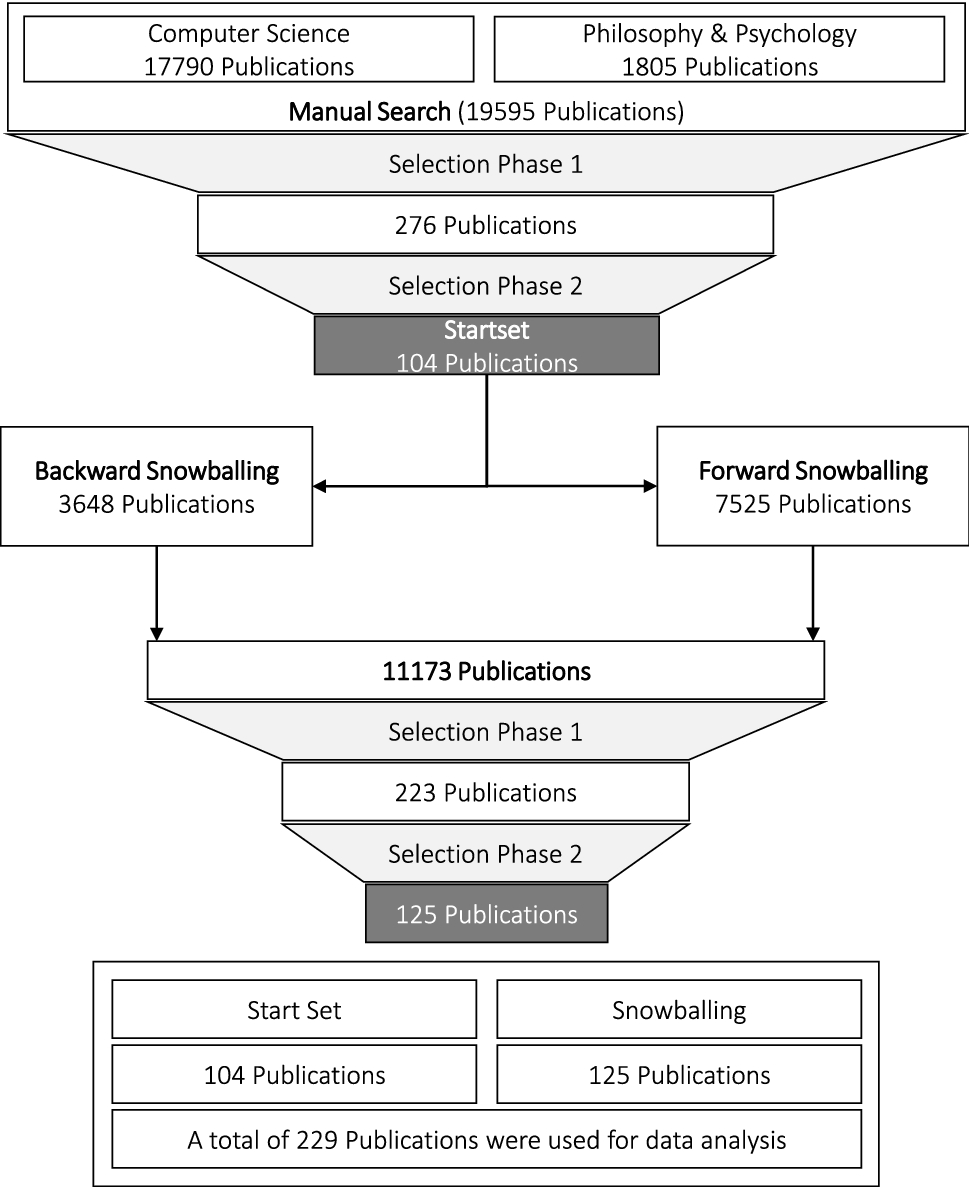
\includegraphics[width=0.3\textwidth]{images/slr_order.png}
        \caption{بررسی ساختار \lr{SLR} انجام شده در این مقاله}
        \label{fig:slrOrder}
    \end{figure}
\end{frame}

\begin{frame}
    \frametitle{دو فاز اصلی انتخاب مقالات این پژوهش}

    \begin{enumerate}
        \item انتخاب مقالات بر مبنای عنوان، چکیده و کلمات کلیدی (همه به صورت
        الگوریتمیک و غیر قابل شناسایی)
        \item انتخاب بر مبنای کل متن و ارزش کلی مقاله
    \end{enumerate}
\end{frame}

\begin{frame}
    \frametitle{چه فرآورده‌ای از پژوهشات انجام شده حاصل شد؟}
    دو بررسی صورت گرفت:
    \begin{enumerate}
        \item بررسی داخلی
        \item بررسی خارجی
    \end{enumerate}
\end{frame}


\begin{frame}
    \frametitle{نیازمندی‌های \lr{NFR} که در \lr{SLR} مورد بررسی قرار گرفته است:}
    ۵۷ نیازمندی غیر عملیاتی:

    \begin{figure}[H]
        \centering
    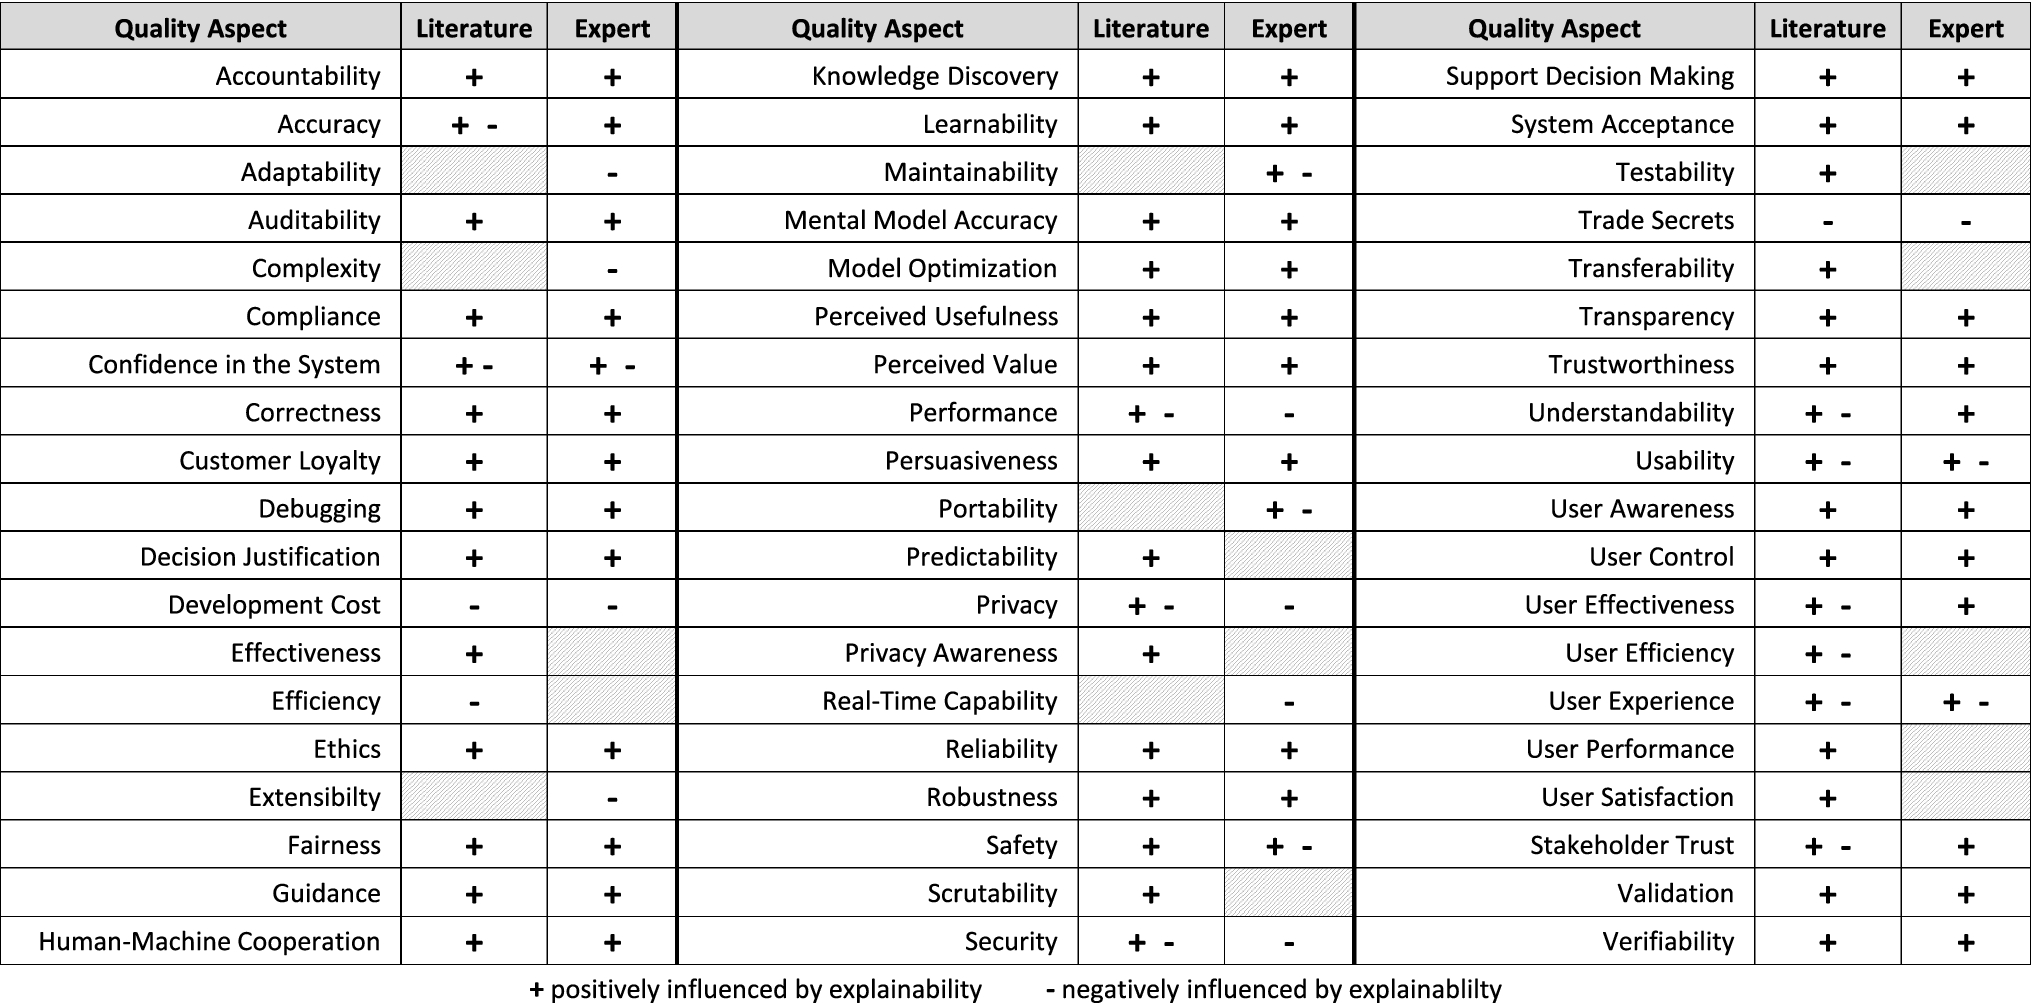
\includegraphics[width=0.9\textwidth]{images/knowledge_catalogue.png}
        \caption{بررسی ساختار \lr{SLR} انجام شده در این مقاله}
        \label{fig:slrOrder}
    \end{figure}
\end{frame}

\end{document}